\documentclass[10pt, conference]{IEEEtran}

	\usepackage{graphicx}
	\usepackage{color}
	\usepackage{epstopdf}
	\usepackage{amsmath}
	\usepackage{float}
	\usepackage[font=small]{caption}
	
	\begin{document}
	\title{Performance Analysis of TCP Variants}
	\author{\IEEEauthorblockN{Yunfan Tian}
	\IEEEauthorblockA{College of Engineering\\
	Northeastern University, MA, 02115\\
	Email: tian.yun@husky.neu.edu\\
	NUID: 001273551}}
	\maketitle
	\begin{abstract}
	This project contains 3 experiments, we use NS-2 to simulate congestion on a simple 6-node network topology with 4 TCP variants and analyze the performance in experiment 1. We also conduct experiment 2 to analyze the fairness between different TCP variants. Then we investigate the influence of queuing disciplines in experiment 3.
	\end{abstract}
	
	
	\section{Introduction}
	Network congestion is the reduced quality of service that occurs when a network node or link is carrying more data than it can handle. Different TCP variants provides different algorithms to control and avoid congestion. In this paper, we present performance and comparative analysis of TCP variants under increasing load and different queuing disciplines.
	
	In experiment 1, we analyze the performance of four TCP variants (Tahoe, Reno, NewReno, Vegas) under increasing CBR load based on throughput, drop rate and latency.
	
	In experiment 2, we analyze the fairness between different TCP variants (Reno/Reno, NewReno/Reno, Vegas/Vegas, NewReno/Vegas) based on throughput, drop rate, and latency.
	
	In experiment 3, we compare the performance of different queuing algorithms (DropTail and RED) under constant CBR load based on throughput and latency.
	
	\section{Methodology}
	\subsection{Network Topology}
	\begin{figure}[H]
		\centering
		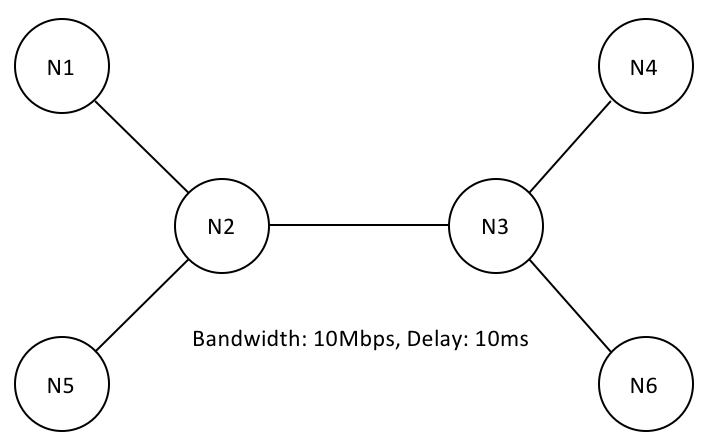
\includegraphics[width=3.45in]{imgs/pic1.png}
		\caption[Optional caption]{Basic Network}
		\label{fig:1}
	\end{figure}
	Fig. \ref{fig:1} shows the basic network for our three experiments. There are 6 nodes and 5 links in network, the bandwidth and delay for each link are configured to \textbf{10Mbps} and \textbf{10ms}.
	
	\subsection{Tools}
	We use NS-2 to conduct all the experiments. NS-2 is a discrete-event computer network simulator, we use it to simulate congestion on network.
	
	Then we use python to analyze the trace files generated by NS-2 and use gnuplot to plot the data.
	
	\subsection{Performance Evaluation}
	We consider throughput, drop rate and latency to evaluate and compare each TCP evaluation. From the trace logs generated by NS-2, we could get the behavior of each packet and then analyze the data flow in network. 
	
	\textit{Throughput} is the amount of data moved successfully from one node to another in given period, measured in \textbf{Mbps}.
	$$ throughput = \frac{packets \ received \times packet \ size}{time} $$
	
	\textit{Drop rate} is the percentage of packets that travel across network fail to reach their destination.
	$$ drop \ rate = \frac{packets \ dropped}{packets \ sent} \ \times \ 100\%$$
	
	\textit{latency} is time interval between packets sent and received, measured in \textbf{s}.
	$$ latency = \frac{\sum packets \ received \times delay}{packets \ received}$$
	
	\subsection{Configurations}
	\textbf{Experiment 1:}
	\begin{figure}[H]
		\centering
		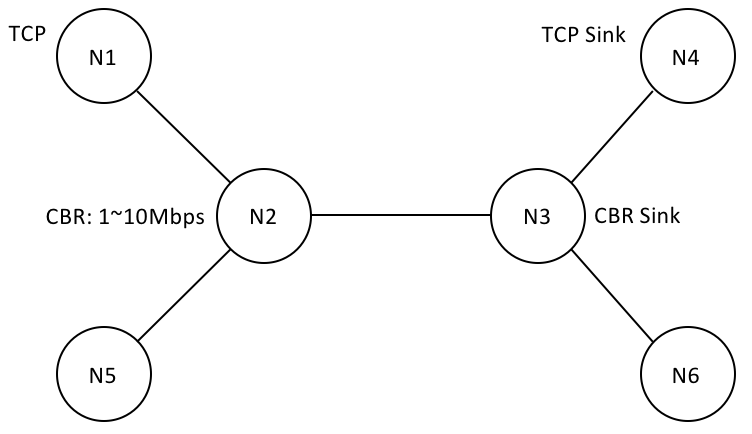
\includegraphics[width=3.45in]{imgs/pic2.png}
		\caption[Optional caption]{Experiment 1}
		\label{fig:2}
	\end{figure}
	Fig. \ref{fig:2} shows the basic configuration in experiment 1. The queuing algorithm of each link is DropTail with a default queue size. The test time is set to 10 seconds. The CBR (Constant Bit Rate) varies from \textbf{1Mbps} to \textbf{10Mbps}. We add CBP from N2 to N3, TCP from N1 to N4, then start N2 and N1 at time 0. Finally, we conducted experiments with TCP Tahoe, Reno, NewReno, Vegas and evaluated the performance.
	\\\\
	\textbf{Experiment 2:}
	\begin{figure}[H]
		\centering
		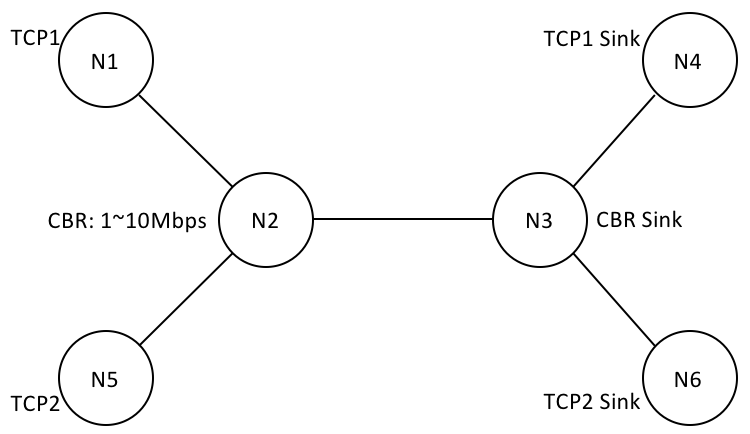
\includegraphics[width=3.45in]{imgs/pic3.png}
		\caption[Optional caption]{Experiment 2}
		\label{fig:3}
	\end{figure}
	Fig. \ref{fig:3} shows the basic configuration in experiment 2. The only difference to experiment 1 is that we add another TCP stream from N5 to N6. Finally, conducted experiments with 4 pairs of TCP variants (Reno/Reno, NewReno/Reno, Vegas/Vegas, NewReno/Vegas) and present comparative analysis.
	\\\\
	\textbf{Experiment 3:}
	\begin{figure}[H]
		\centering
		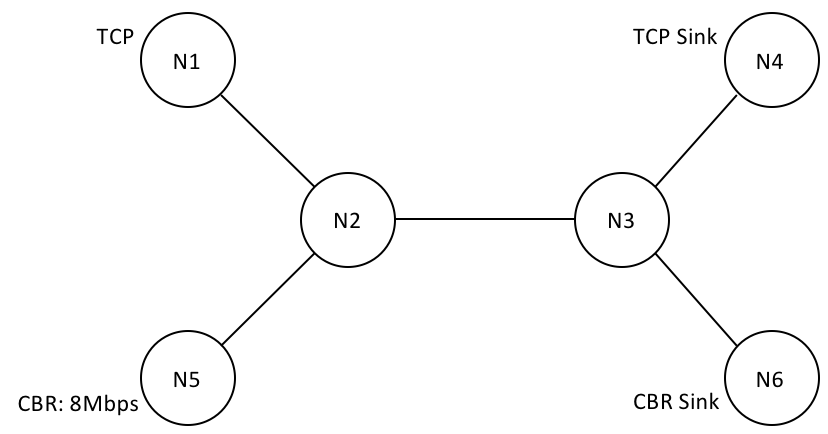
\includegraphics[width=3.45in]{imgs/pic4.png}
		\caption[Optional caption]{Experiment 3}
		\label{fig:4}
	\end{figure}
	Fig. \ref{fig:4} shows the basic configuration in experiment 3. We add TCP from N1 to N4, CBR from N5 to N6. The link queuing algorithm is DropTail or Random Early Drop (RED), and the TCP variant is Reno or Sack. We set test time to 20s, queue limit to 10 and CBR to 8Mbps. Finally, we start CBR at \textbf{0s} and TCP at \textbf{4s}, and then monitor throughput and latency of TCP stream over 20 second period.
	
	\section{Experiment 1 Result Analysis}
	\subsection{Throughput}
	\begin{figure}[H]
		\centering
		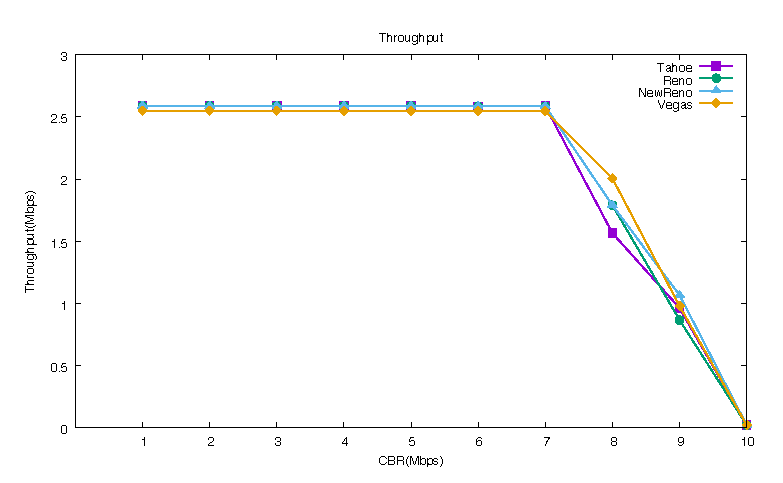
\includegraphics[width=3.45in]{imgs/exp1_throughput.eps}
		\caption[Optional caption]{Throughput}
		\label{fig:5}
	\end{figure}
	For CBR $\le$ 7Mbps, the throughput of of all TCP variants stay stable around 2.6Mbps. Vega's throughput is a little less than the other three. After CBR exceed 5 Mbps, congestion raises, and all TCP variants begin to drop. However, Vega has better overall performance than the other three, Tahoe has least throughput. That's because Vegas conducts congestion detection at beginning, and when network become congested, the pre-detection help to keep a higher throughput.
	\subsection{Drop Rate}
	\begin{figure}[H]
		\centering
		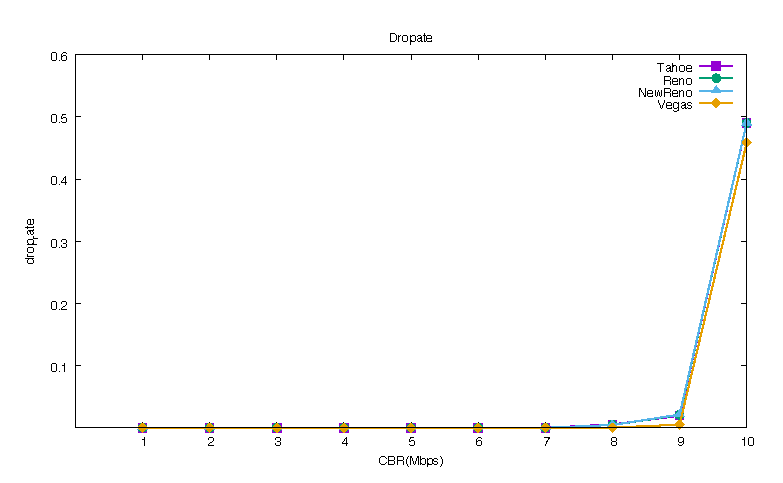
\includegraphics[width=3.45in]{imgs/exp1_droprate.eps}
		\caption[Optional caption]{Drop Rate}
		\label{fig:6}
	\end{figure}
	After the congestion begin, Vegas has best performance compare the other three. All TCP variants are sensitive to the congestion, but Vegas has 50\% less drop rate compare to others when CBR is 9Mbps.
	\subsection{Latency}
	\begin{figure}[H]
		\centering
		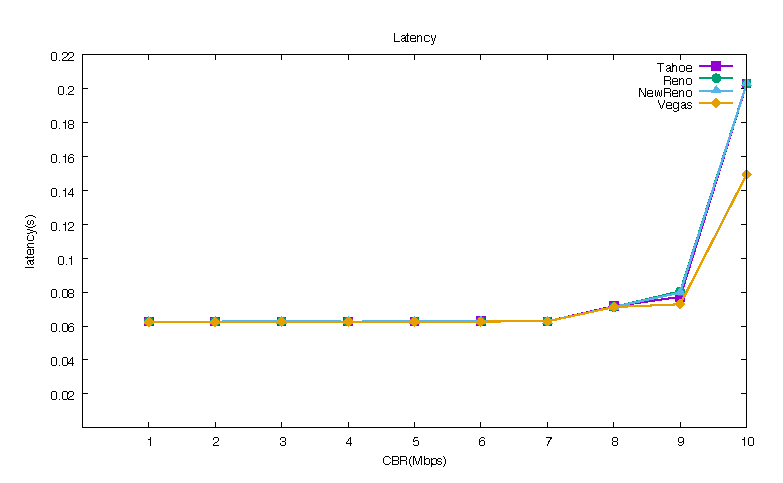
\includegraphics[width=3.45in]{imgs/exp1_latency.eps}
		\caption[Optional caption]{Latency}
		\label{fig:7}
	\end{figure}
	All TCP variants have same latency before congestion, but Vegas still remains fairly low latency under congestion. As CBR increases to the bandwidth limit (10Mbps), Vegas keeps 0.15s latency, but other variants reach 0.2s.
	
	\section{Experiment 2 Result Analysis}
	\subsection{Reno vs Reno}
	\begin{figure}[H]
		\centering
		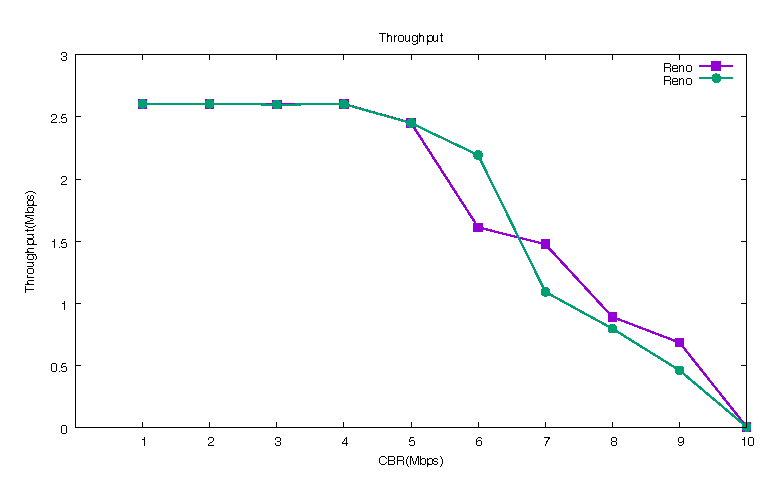
\includegraphics[width=3.45in]{imgs/exp2_tp_Reno_Reno.eps}
		\caption[Optional caption]{Throughput}
		\label{fig:8}
	\end{figure}
	\begin{figure}[H]
		\centering
		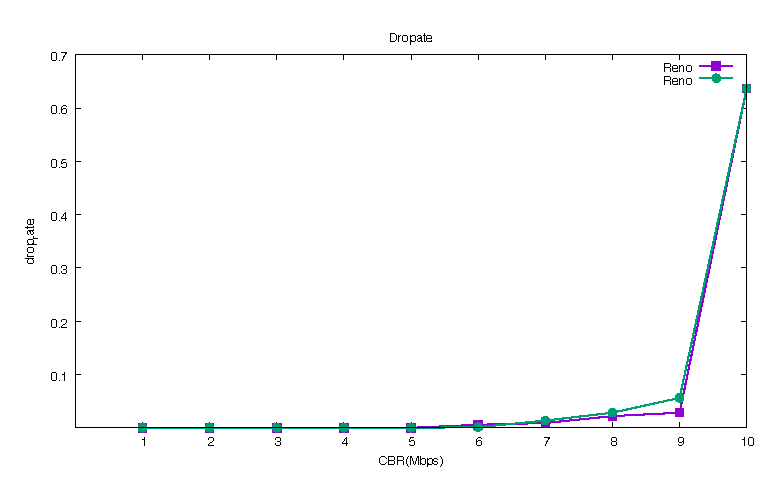
\includegraphics[width=3.45in]{imgs/exp2_dr_Reno_Reno.eps}
		\caption[Optional caption]{Drop rate}
		\label{fig:9}
	\end{figure}
	\begin{figure}[H]
		\centering
		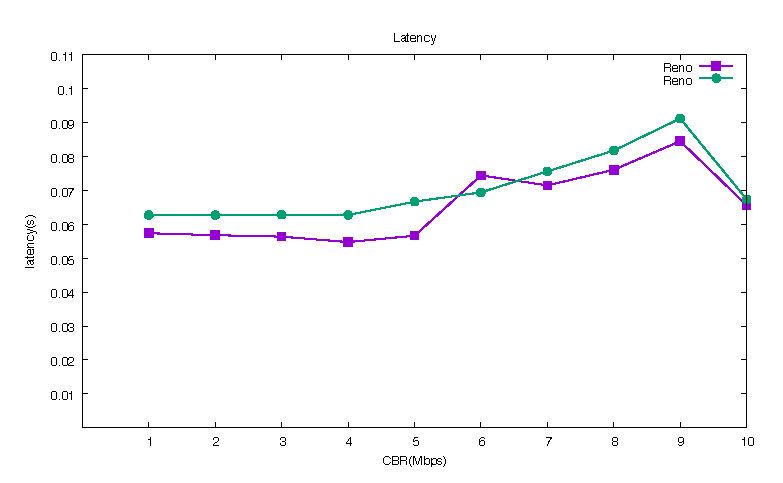
\includegraphics[width=3.45in]{imgs/exp2_la_Reno_Reno.eps}
		\caption[Optional caption]{latency}
		\label{fig:10}
	\end{figure}
	Fig. \ref{fig:8}, Fig, \ref{fig:9} and Fig. \ref{fig:10} show the comparison of throughput, drop rate and latency between Reno and Reno. In Fig. \ref{fig:8} and Fig. \ref{fig:9}, \textit{throughput} and \textit{Drop rate} value oscillated back and forth but keep close in the same track as CBR increased from 0 to 10Mbps. The oscillation is acceptable. In Fig. \ref{fig:10}, One TCP Reno agent has a little lower latency than the other. Thus two TCP Reno maintain fair for throughput and drop rate.
	
	\subsection{NewReno vs Reno}
	\begin{figure}[H]
		\centering
		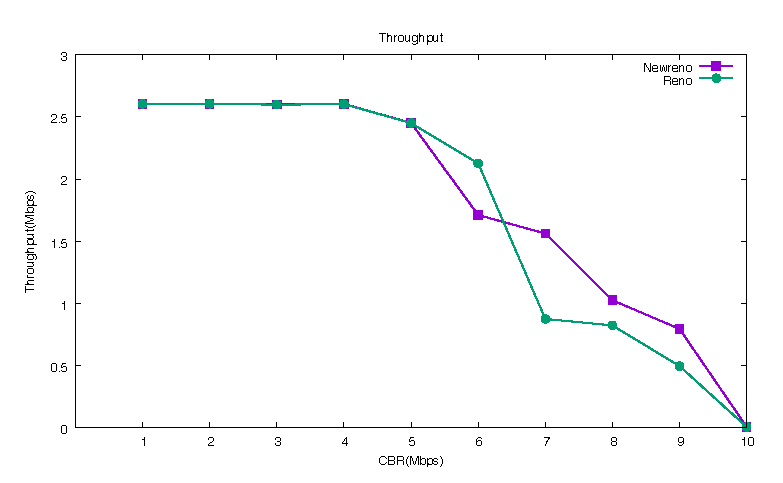
\includegraphics[width=3.45in]{imgs/exp2_tp_Newreno_Reno.eps}
		\caption[Optional caption]{Throughput}
		\label{fig:11}
	\end{figure}
	\begin{figure}[H]
		\centering
		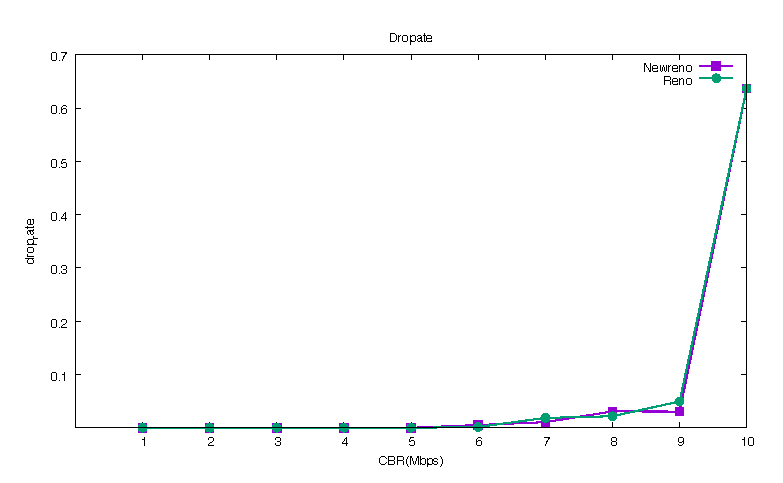
\includegraphics[width=3.45in]{imgs/exp2_dr_Newreno_Reno.eps}
		\caption[Optional caption]{Drop rate}
		\label{fig:12}
	\end{figure}
	\begin{figure}[H]
		\centering
		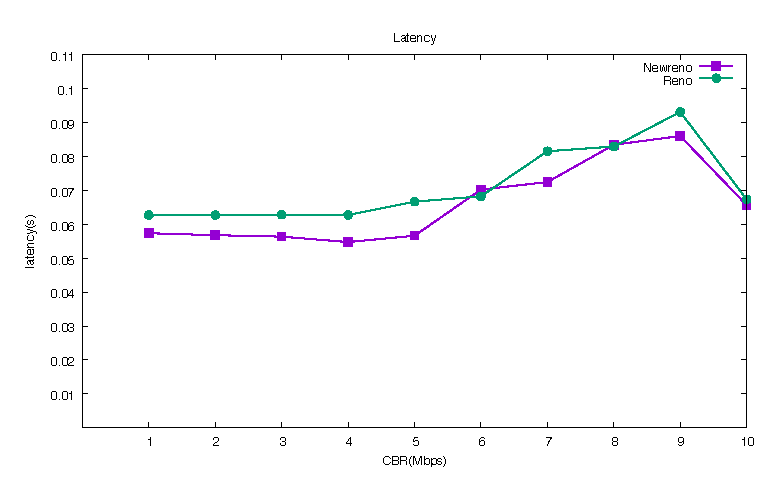
\includegraphics[width=3.45in]{imgs/exp2_la_Newreno_Reno.eps}
		\caption[Optional caption]{latency}
		\label{fig:13}
	\end{figure}
	Fig. \ref{fig:11}, Fig, \ref{fig:12} and Fig. \ref{fig:13} show the comparison of throughput, drop rate and latency between NewReno and Reno. In these three figures, the value oscillated back and forth but keep close in the same track as CBR increased from 0 to 10Mbps. The oscillation is acceptable. Thus,  NewReno and Reno maintain fair for all three features.
	
	\subsection{Vegas vs Vegas}
	\begin{figure}[H]
		\centering
		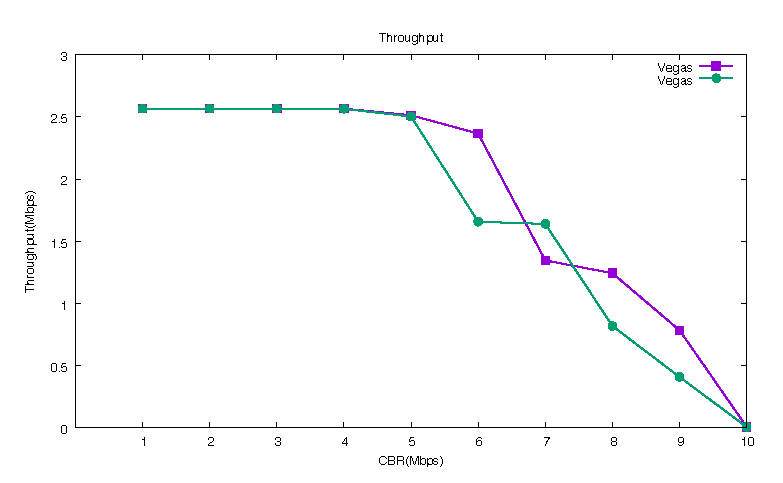
\includegraphics[width=3.45in]{imgs/exp2_tp_Vegas_Vegas.eps}
		\caption[Optional caption]{Throughput}
		\label{fig:14}
	\end{figure}
	\begin{figure}[H]
		\centering
		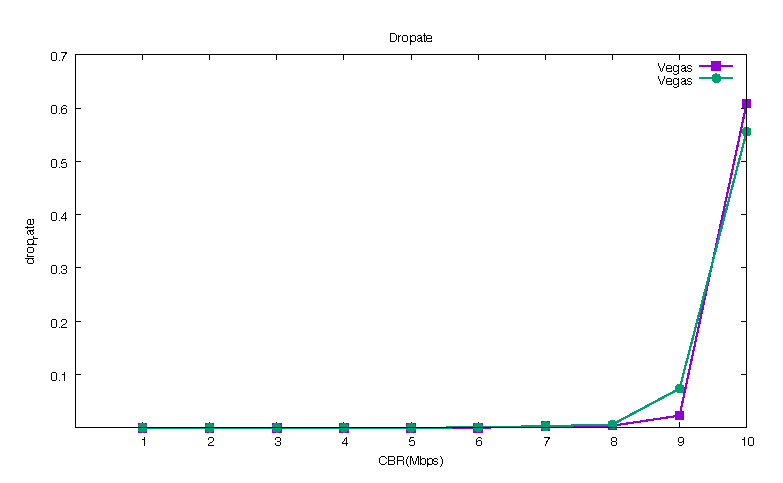
\includegraphics[width=3.45in]{imgs/exp2_dr_Vegas_Vegas.eps}
		\caption[Optional caption]{Drop rate}
		\label{fig:15}
	\end{figure}
	\begin{figure}[H]
		\centering
		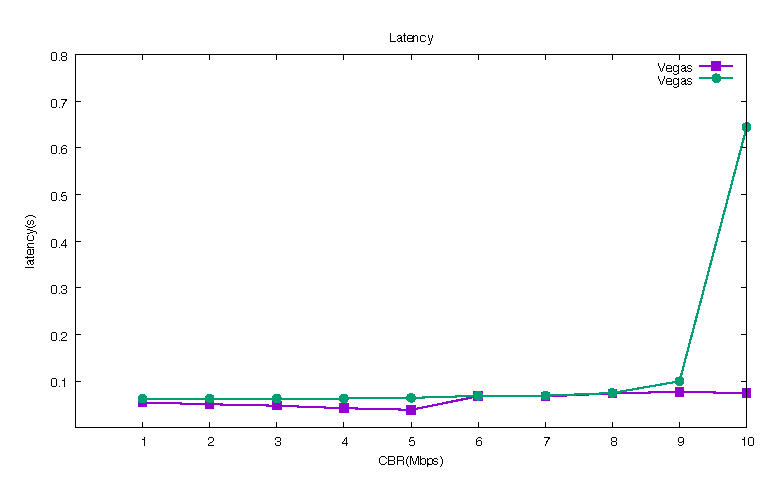
\includegraphics[width=3.45in]{imgs/exp2_la_Vegas_Vegas.eps}
		\caption[Optional caption]{latency}
		\label{fig:16}
	\end{figure}
	Fig. \ref{fig:14}, Fig, \ref{fig:15} and Fig. \ref{fig:16} show the comparison of throughput, drop rate and latency between Vegas and Vegas. In Fig. \ref{fig:14} and Fig, \ref{fig:15}, the throughput and drop rate value oscillated back and forth but keep close in the same track as CBR increased from 0 to 10Mbps. The oscillation is acceptable.
	However, in Fig. \ref{fig:16}, one Vegas agent's latency differed much from another. When CBR reached 10Mbps, one Vegas agent has 0.65s latency, but another still maintain 0.08s. Thus two Vegas agents didn't keep fair. That's because Vegas provide congestion detection mechanism.
	
	\subsection{NewReno vs Vegas}
	\begin{figure}[H]
		\centering
		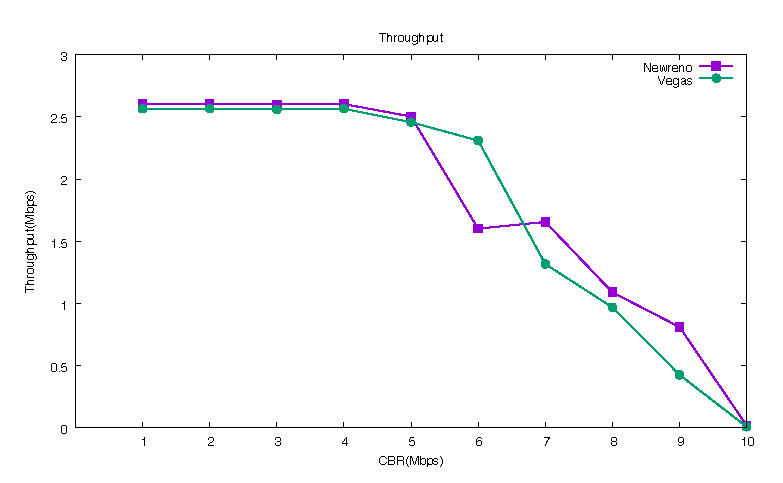
\includegraphics[width=3.45in]{imgs/exp2_tp_Newreno_Vegas.eps}
		\caption[Optional caption]{Throughput}
		\label{fig:17}
	\end{figure}
	\begin{figure}[H]
		\centering
		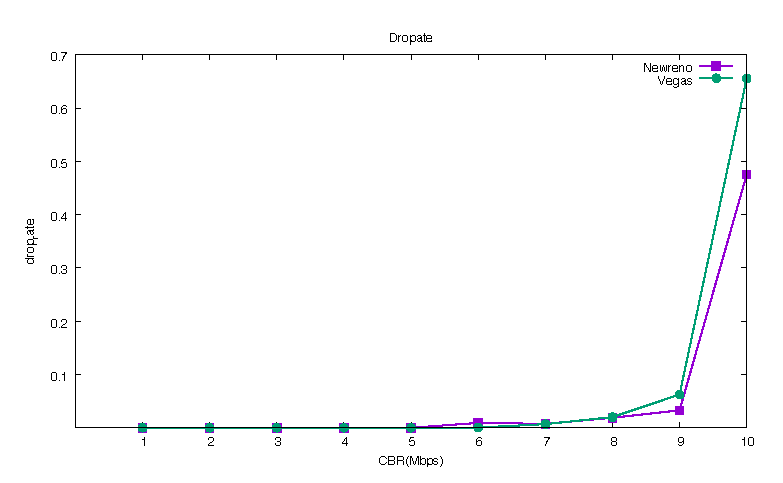
\includegraphics[width=3.45in]{imgs/exp2_dr_Newreno_Vegas.eps}
		\caption[Optional caption]{Drop rate}
		\label{fig:18}
	\end{figure}
	\begin{figure}[H]
		\centering
		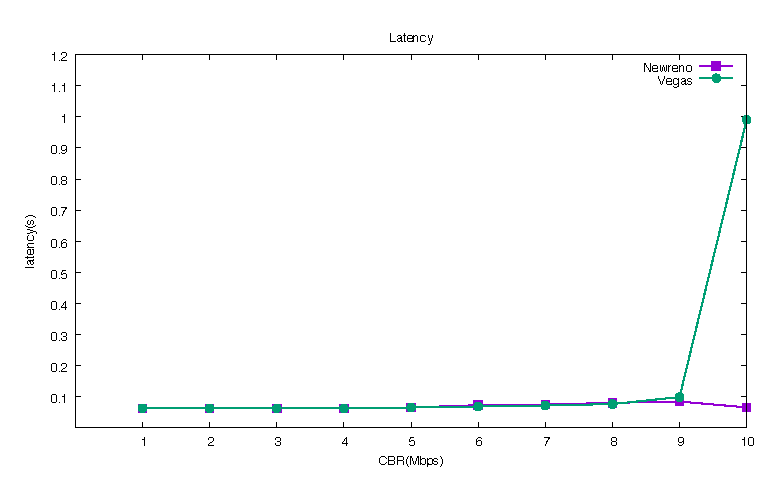
\includegraphics[width=3.45in]{imgs/exp2_la_Newreno_Vegas.eps}
		\caption[Optional caption]{latency}
		\label{fig:19}
	\end{figure}
	Fig.\ref{fig:17}, Fig, \ref{fig:18} and Fig. \ref{fig:19} show the comparison of throughput, drop rate and latency between NewReno and Vegas. In Fig. \ref{fig:17}, the throughput value oscillated back and forth but keep close in the same track as CBR increased from 0 to 10Mbps. The oscillation is acceptable.
	
	However, in Fig. \ref{fig:18} and Fig. \ref{fig:19}, NewReno agent's drop rate and latency differed much from Vegas. NewReno has a lower drop rate under congestion. When CBR reached 10Mbps, Vegas has 1s latency, but NewReno maintain 0.08s. Thus NewReno and Vegas agents didn't keep fair. That's because when NewReno is dominate, Vegas supposed the network is congested and reduced its sending rate.
	\section{Experiment 3 Result Analysis}
	\subsection{Throughput}
	\begin{figure}[H]
		\centering
		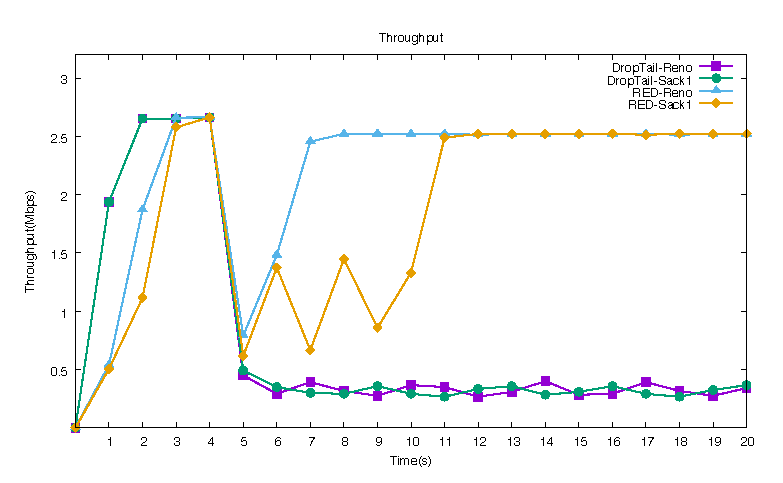
\includegraphics[width=3.45in]{imgs/exp3_throughput.eps}
		\caption[Optional caption]{Throughput}
		\label{fig:20}
	\end{figure}
	Before CBR added at 4s, DropTail has better performance than RED and achieves stability faster. When CBR added, all 4 TCP throughput drop dramatically. DropTail finally oscillated around 0.35Mbps since 5s. RED-Reno increased to 2.5Mbps since 7s and remain stable. RED-Sack oscillated and increased to 2.5Mbps since 11s and remain stable.
	
	RED queuing algorithm generally has a better performance than DropTail under congestion. Each queuing discipline didn't provide fair bandwidth to each flow. RED recovers faster from throughput drop and has a better utilization of bandwidth.

	\subsection{Latency}
	\begin{figure}[H]
		\centering
		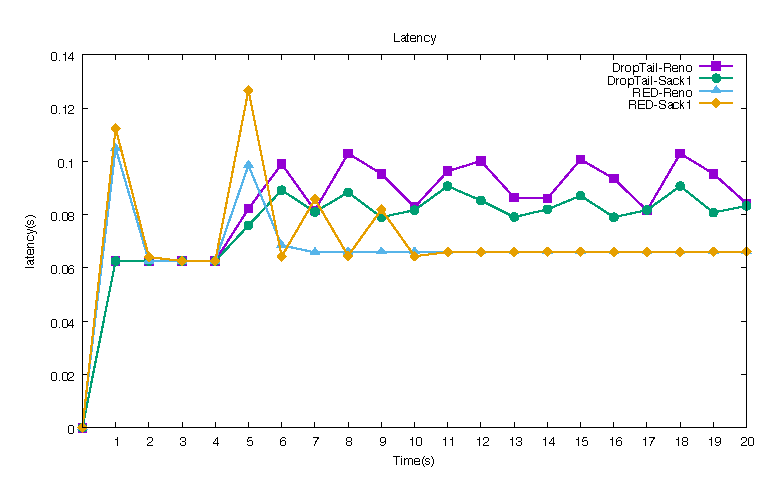
\includegraphics[width=3.45in]{imgs/exp3_latency.eps}
		\caption[Optional caption]{Latency}
		\label{fig:21}
	\end{figure}
	We calculated average latency in each second and compare.
	
	Before CBR added at 4s, DropTail achieves stability faster and both queuing algorithm have same 0.06s latency. When CBR added, all 4 TCP latency increase dramatically. DropTail finally oscillated around 0.09s since 6s. Sack has lower latency than Reno. RED-Reno drops to 0.06s since 7s and remain stable. RED-Sack oscillated and drops to 0.06s since 11s and remain stable.
	
	RED queuing algorithm generally has a better performance of latency than DropTail under congestion. RED is a good idea with SACK because it has low latency with high throughput. The only problem is RED-Sack takes more time to achieve stability.
		
	\section{Conclusion}
	In this paper, we simulate different TCP variants and queuing disciplines under congestion with NS-2 and analyze the performance of them based on throughput, packets drop rate and latency. From these 3 experiments, 
	we can conclude that:
	\begin{enumerate}
		\item For single TCP agent, Vegas has better performance than Tahoe, Reno and NewReno in throughput, drop rate and latency.
		\item For two TCP agents in same network, they may perform unfair to each other. Reno is fair to Reno; NewReno is fair to Reno. Vegas is not fair to Vegas in latency; NewReno is not fair to Vegas in drop rate and latency.
		\item RED is a good idea with SACK because it provides low latency with high throughput. The only problem is RED-Sack takes more time to achieve stability.
	\end{enumerate}
	
	\begin{thebibliography}{1}
	\bibitem{tcp:sim}
	Kevin Fall and Sally Floyd, \emph{Simulation-based Comparisons of Tahoe, Reno, and SACK TCP}.
	
	\bibitem{tcp:congestion}
	Wikipedia, \emph{Network congestion}, https://en.wikipedia.org/wiki/Network\_congestion
	
	\end{thebibliography}
	
	\end{document}